\chapter{Methodology and Technical Approach}
\label{ch:method}

This chapter is the scientific core of the report. It is written to be reproducible: another researcher should be able to re-implement the scoring workflow, regenerate tables, and relaunch the dashboard from the provided schema and code.

\section{General Solution Architecture}
\label{sec:arch}

The system follows one short pipeline (Figure~\ref{fig:pipeline}):
\textbf{Input data} $\rightarrow$ \textbf{Processing} $\rightarrow$ \textbf{RAG}
$\rightarrow$ \textbf{Dashboard}.

\begin{figure}[htbp]
\centering
\begin{tikzpicture}[
  box/.style={draw=aivNavy, line width=0.8pt, rounded corners=2pt, align=center,
              font=\small\bfseries, fill=aivBox, minimum width=3.35cm,
              minimum height=1.0cm, inner sep=3pt},
  arr/.style={-{Latex}, thick, aivNavy}]
  \node[box] (in) {Input data};
  \node[box, right=0.55cm of in] (proc) {Processing};
  \node[box, right=0.55cm of proc] (rag) {RAG};
  \node[box, right=0.55cm of rag] (out) {Dashboard};
  \draw[arr] (in) -- (proc);
  \draw[arr] (proc) -- (rag);
  \draw[arr] (rag) -- (out);
\end{tikzpicture}

\vspace{0.35em}
{\footnotesize
\begin{tabular}{@{}llll@{}}
Input: laws, papers, JSON &
Process: clean, score, chunk &
RAG: retrieve + cite &
UI: maps, compare, Q\&A \\
\end{tabular}}
\caption{Overall project pipeline (brief). Source: author.}
\label{fig:pipeline}
\end{figure}

\begin{table}[htbp]
\centering
\caption{Pipeline stages (brief description)}
\label{tab:arch}
\begin{tabular}{@{}p{2.6cm}p{9.0cm}@{}}
\toprule
\textbf{Stage} & \textbf{Role} \\
\midrule
Input data & Public agency documents, literature, and curated country records \\
Processing & Screening, seven-theme scoring, chunking, provenance logging \\
RAG & Retrieve relevant passages and produce grounded, cited answers \\
Dashboard & React/Streamlit views: map, radar, themes, RAG Assistant, export \\
\bottomrule
\end{tabular}
\end{table}

In short: curated data feed the RAG module; RAG evidence supports exploration in the
dashboard (Chapter~\ref{ch:rag}). Full application code is available at
\newline\noindent\repoLink{}.

\section{Literature Search and Inclusion Protocol}
\label{sec:search}

\subsection{Databases and Regulatory Sources}

Search covered PubMed, Scopus, IEEE Xplore, Google Scholar, and SSRN, complemented by FDA, EMA, MHRA, NMPA, WHO, OECD, and national AI strategy portals. Inclusion emphasized 2018--2026 publications addressing AI regulation, compliance, or ethics in healthcare, plus foundational pre-2018 frameworks still in force (e.g., IMDRF 2014, HIPAA).

\subsection{Query Design}

Representative query families included: ``AI healthcare regulation'', ``SaMD compliance'', ``health data governance'', ``algorithmic transparency medicine'', ``EU AI Act medical device'', and ``post-market surveillance AI''. Snowballing from key reviews (e.g., device-approval comparisons, ethics surveys) complemented keyword search~\cite{muehlematter2021,jobin2019}.

\subsection{Screening Logic}

Titles/abstracts were screened for healthcare + AI + regulatory/ethical relevance. Full texts informed theme narratives. Grey literature (agency PDFs) was admitted when it constituted primary law or official guidance. Informal encyclopedias and blogs may inform discovery but do not justify score cells or bibliographic claims.

\section{Seven-Theme Scoring Ontology}
\label{sec:ontology}

\begin{table}[htbp]
\centering
\caption{Compliance themes used for jurisdictional scoring}
\label{tab:themes}
\begin{tabularx}{\textwidth}{@{}c X@{}}
\toprule
\textbf{ID} & \textbf{Theme} \\
\midrule
    1 & Data Privacy \& Governance \\
    2 & Clinical Validation \& Safety \\
    3 & Regulatory Approval Process \\
    4 & Algorithmic Transparency \\
    5 & Ethical Considerations \\
    6 & Post-Market Surveillance \\
    7 & Liability \& Accountability \\
\bottomrule
\end{tabularx}
\end{table}

Each theme is scored on an integer scale from 1 (minimal formalization / capacity) to 10 (mature, AI-aware, enforceable framework). Scores are comparative indicators combining: existence of AI-relevant rules; enforceability; agency capacity signals; and alignment with international good practice (IMDRF, GMLP, WHO ethics). Higher is not automatically ``better for innovation''; some high scores reflect stringent precaution.

\subsection{Calibration Rules}

\begin{itemize}[noitemsep]
  \item Prefer primary legal texts over secondary commentary when assigning scores;
  \item Separate ``law on the books'' from evident implementation capacity when narratives disagree;
  \item Record device-approval counts as a complementary throughput metric, not a quality proxy alone;
  \item Document uncertainty in country narrative fields (\texttt{challenges}, \texttt{notable\_developments}).
\end{itemize}

\section{Dataset Schema and Curation Workflow}
\label{sec:schema}

The canonical file \texttt{data/compliance\_dataset.json} contains:
\begin{itemize}[noitemsep]
  \item \texttt{metadata} --- title, version, theme list, sources;
  \item \texttt{countries} --- array of jurisdictional objects;
  \item \texttt{global\_trends} --- structured trend cards;
  \item \texttt{key\_references} --- bibliographic pointers.
\end{itemize}

Country objects include identifiers (\texttt{country}, \texttt{iso\_code}, \texttt{region}), institutional fields (\texttt{regulatory\_body}, privacy law, AI-specific regulation, medical-device framework), narrative dimensions aligned to themes, \texttt{key\_legislations}, \texttt{maturity\_level}, \texttt{year\_first\_ai\_regulation}, \texttt{num\_ai\_devices\_approved}, and \texttt{themes\_scores}.

\begin{equation}
\label{eq:composite}
S_c = \frac{1}{7} \sum_{t=1}^{7} s_{c,t}
\end{equation}
where $s_{c,t} \in [1,10]$ is the score of country $c$ on theme $t$, and $S_c$ is the unweighted composite used for choropleth coloring unless a user applies filters.
The mean is unweighted so that no single theme (e.g., privacy or approval throughput) dominates the default ranking; theme-level scores and alternative weightings in Section~\ref{sec:sensitivity} expose policy trade-offs explicitly.

\section{NLP Pipeline Design (Scale-Up Path)}
\label{sec:nlp}

Phase~1 proposed an assembly-line NLP approach. The draft methodology retained for reproducibility is:

\subsection{Data Collection and Ingestion}

Sources include official HTML/PDF portals and bibliographic APIs. Acquisition scripts should log URL, access date, and checksum. Update frequency for a production system would be monthly for agency newsrooms and event-driven for major legislative acts.

\subsection{Preprocessing}

\begin{enumerate}[noitemsep]
  \item PDF/HTML text extraction;
  \item language detection and optional translation for indexing;
  \item normalization (Unicode, hyphenation repair);
  \item segmentation into articles/sections/clauses;
  \item metadata tagging (jurisdiction, instrument type, date).
\end{enumerate}

\subsection{Feature Extraction}

Lexical baselines (TF--IDF) provide interpretable sparse features. Dense embeddings (e.g., domain-adapted BERT) capture semantic similarity between clauses on ``clinical validation'' or ``human oversight.'' Equation~\eqref{eq:embed} denotes sentence embedding $\mathbf{e}_i$ for segment $i$:
\begin{equation}
\label{eq:embed}
\mathbf{e}_i = f_\theta(x_i) \in \mathbb{R}^d
\end{equation}
with encoder parameters $\theta$ frozen or fine-tuned depending on labeled data availability.

\subsection{Classification and HITL}

Draft labels map segments to themes and coarse risk cues. Human-in-the-loop review is mandatory before scores change: NLP accelerates scanning; experts remain accountable for regulatory meaning.

\section{Dashboard Implementation}
\label{sec:dashimpl}

\subsection{Technology Stack}

\begin{table}[htbp]
\centering
\caption{Implementation stack}
\label{tab:stack}
\begin{tabular}{@{}ll@{}}
\toprule
\textbf{Component} & \textbf{Technology} \\
\midrule
Analytics prototype & Streamlit + Plotly + Pandas \\
Presentation web app & React + Recharts + react-simple-maps \\
Data store & Versioned JSON \\
Report generation & LaTeX, fpdf2, python-pptx \\
Runtime & Python 3.9+, Node.js (web) \\
\bottomrule
\end{tabular}
\end{table}

\subsection{Information Architecture}

Primary views: World Map; Country Comparison; Theme Analysis; Global Trends; Country Details; AI Use Cases \& Trends; Literature Review. Filters include region, maturity, and minimum theme score. CSV export supports external audit of the exact filtered subset.

\subsection{Use-Case Readiness Model}

For clinical domains $u$ (radiology, pathology, genomics, drug discovery), a derived readiness score uses theme weights $w_{u,t}$:
\begin{equation}
\label{eq:usecase}
R_{c,u} = \sum_{t=1}^{7} w_{u,t} \, s_{c,t}
\quad \text{with} \quad \sum_t w_{u,t} = 1, \; w_{u,t} \ge 0.
\end{equation}
Radiology emphasizes clinical validation and post-market surveillance; genomics emphasizes privacy; drug discovery emphasizes approval process and transparency. Weights are disclosed in the UI to avoid black-box rankings.

\subsection{Evaluation Metrics for the Software Artifact}

Unlike a single predictive model, evaluation combines:
\begin{itemize}[noitemsep]
  \item \textbf{Coverage:} 20/20 countries with complete theme vectors;
  \item \textbf{Consistency:} schema validation and non-null critical fields;
  \item \textbf{Usability:} task-based walkthroughs (compare two countries; identify lowest liability scores);
  \item \textbf{Reproducibility:} one-command local launch;
  \item \textbf{Traceability:} each narrative linked to legislation lists and bibliography.
\end{itemize}

\section{Baselines and Alternatives Considered}
\label{sec:baselines}

Methodological alternatives rejected or deferred:
\begin{itemize}[noitemsep]
  \item \textbf{Pure qualitative review:} insufficiently actionable for comparative dashboards;
  \item \textbf{Fully automated scraping without curation:} high factual risk for legal text;
  \item \textbf{Single composite index without themes:} hides policy trade-offs (e.g., high approvals vs weak transparency);
  \item \textbf{Closed commercial data only:} conflicts with academic reproducibility.
\end{itemize}
The chosen hybrid---expert curation + interactive analytics + NLP-ready schema---optimizes for scientific reproducibility and practical stakeholder use.

\section{Environment, Versioning, and Reproducibility}
\label{sec:repro}

Code and data for the interactive dashboard are published at
\newline\noindent\repoLink{}
(\texttt{app.py}, \texttt{requirements.txt}, \texttt{literature\_review.md}, and \texttt{data/compliance\_dataset.json}).
Dependencies are pinned via \texttt{requirements.txt}. Dataset \texttt{version} and \texttt{last\_updated} fields support audit trails. Listing~\ref{lst:launch} shows the canonical Streamlit launch command.

\begin{lstlisting}[caption={Launching the Streamlit compliance dashboard},label={lst:launch}]
pip install -r requirements.txt
python -m streamlit run app.py
# open http://localhost:8501
\end{lstlisting}


\section{Extended Methodological Documentation}
\label{sec:method-extended}

The subsections below provide reproducible detail required by the aivancity methodology guidelines (rubrics, worked examples, and UI structure).

\subsection{Detailed Scoring Rubric by Theme}
\label{sec:rubric}

To improve reproducibility, Table~\ref{tab:rubric} summarizes ordinal anchors used during curation. Intermediate scores (e.g., 5--6) indicate partial AI-specificity or uneven enforcement capacity.

\begin{table}[htbp]
\centering
\caption{Simplified ordinal anchors for theme scores (1--10)}
\label{tab:rubric}
\begin{tabular}{@{}p{2.4cm}p{4.0cm}p{4.2cm}@{}}
\toprule
\textbf{Theme} & \textbf{Low (1--3)} & \textbf{High (8--10)} \\
\midrule
Data privacy & Minimal health-data rules; weak enforcement & Comprehensive law + health-sensitive rules + transfer tools \\
Clinical validation & No AI-aware evidence expectations & Clear AI evidence guidance, bias/subgroup expectations, RWE pathways \\
Approval process & General device law only, unclear AI path & Explicit AI/SaMD pathways, sandboxes, predictable review \\
Transparency & No documentation/logging expectations & Binding technical docs, logging, user notices, oversight duties \\
Ethics & Absent or purely rhetorical principles & Institutionalized ethics tools linked to procurement/oversight \\
Post-market & Paper adverse-event systems only & Lifecycle monitoring, update governance, AI-aware vigilance \\
Liability & No AI-relevant clarity & Explicit reforms or mature case guidance allocating responsibility \\
\bottomrule
\end{tabular}
\end{table}

\subsection{Worked Example of Score Assignment}
\label{sec:worked}

Consider a stylized comparison between a jurisdiction with a binding high-risk AI law layered on MDR/GDPR versus one with high device throughput but sectoral privacy and voluntary ethics toolkits. The first may score higher on transparency, ethics, and privacy even if the second reports more device authorizations. Equation~\eqref{eq:composite} deliberately uses an unweighted mean so that no single theme dominates; users who need policy-weighted views can recompute $S_c$ externally from exported CSV.

\subsection{Streamlit Application Structure}
\label{sec:streamlit}

The Streamlit prototype loads JSON at startup, normalizes records into a Pandas DataFrame, and renders:
\begin{itemize}[noitemsep]
  \item sidebar filters (region, maturity, minimum theme thresholds);
  \item executive KPI cards (top/bottom composites, largest theme gaps);
  \item choropleth mapping of $S_c$;
  \item pairwise comparison bars and radar charts;
  \item theme heatmaps and distributions;
  \item trend cards with adoption metadata;
  \item country narrative accordion pages;
  \item derived use-case readiness charts;
  \item embedded literature markdown browser.
\end{itemize}
Custom CSS provides a presentation-ready layout for stakeholder demos. Because all data are local, the demo requires no API keys---an intentional constraint for offline and reproducible deployment.

\subsection{React Presentation Layer}
\label{sec:react}

A React + Vite application mirrors the analytical pages with a Power-BI-inspired layout (header, slicers, KPI tiles, multi-visual pages). Libraries include Recharts for plots and react-simple-maps for geospatial views. A sync script copies the JSON dataset into the web public folder to keep both UIs aligned. This dual-implementation strategy separates rapid scientific iteration (Python) from polished stakeholder storytelling (TypeScript/React).

% --- AI techniques overview (brief; full technical details in Chapters 5 and 6) ---
\section{Artificial Intelligence Techniques Applied in This Project}
\label{sec:ai}

This section consolidates the AI methods that underwrite the project---beyond
jurisdiction scoring alone---so that the defence can clearly separate
\emph{domain content} (healthcare regulation) from \emph{technical AI methods}
(representation learning, retrieval, interactive analytics).

\subsection{Role of AI in the Overall System}
\label{sec:ai-role}

Artificial intelligence appears at three layers:
\begin{enumerate}[noitemsep]
  \item \textbf{Object of study:} AI/ML-enabled SaMD and clinical decision support as
        regulated artefacts~\cite{topol2019,rajpurkar2022,esteva2019};
  \item \textbf{Analytical methods:} ordinal multi-theme scoring, composite indices, and
        use-case readiness models (Chapter~\ref{ch:method});
  \item \textbf{Engineering methods:} NLP embeddings, hybrid retrieval, RAG, and
        interactive visualization (Chapter~\ref{ch:rag}).
\end{enumerate}

\subsection{Representation Learning for Regulatory Text}
\label{sec:ai-rep}

Transformer encoders map variable-length text $x$ to dense vectors
$\mathbf{e}=f_\theta(x)\in\mathbb{R}^{d}$~\cite{vaswani2017,devlin2019}. Self-attention
allows the model to relate distant tokens (e.g., ``high-risk'' and ``medical device'')
without handcrafted features. Domain-adapted checkpoints such as SciBERT improve
scientific vocabulary coverage~\cite{beltagy2019}. In this project, embeddings support:
\begin{itemize}[noitemsep]
  \item semantic search over guidance documents;
  \item clustering of similar clauses across jurisdictions;
  \item future supervised theme classification with human-in-the-loop labels.
\end{itemize}

\subsection{Classical and Hybrid Information Retrieval}
\label{sec:ai-ir}

Before neural retrieval, BM25 provides a strong sparse baseline that excels at exact
identifiers. Hybrid fusion combines BM25 with dense cosine similarity
(Section~\ref{sec:rag-rrf}, Equation~\eqref{eq:rag-def}). This design choice is deliberate for
defence: it shows mastery of both classical IR and modern dense retrieval rather than
blind reliance on an API chatbot.

\subsection{Retrieval-Augmented Generation}
\label{sec:ai-rag-brief}

RAG conditions a generator on retrieved evidence~\cite{lewis2020rag}, reducing
hallucination risk for statute-sensitive questions. The project treats RAG as a
\emph{systems} contribution: corpus design, chunk metadata, citation policy, and
dashboard integration matter as much as the choice of LLM backbone.

\subsection{Interactive Analytics as Human--AI Collaboration}
\label{sec:ai-hci}

Dashboards are not ``AI'' in the narrow sense of learned predictors, yet they are
central to responsible AI tooling: they externalize model/score assumptions, support
counterfactual theme weighting, and keep humans in control of high-stakes interpretations.
The React and Streamlit interfaces operationalize HITL principles advocated in clinical
AI ethics literature~\cite{char2018,mittelstadt2019}.

\subsection{Deep Learning Context for Clinical AI Regulation}
\label{sec:ai-clinical-dl}

Understanding why regulators struggle with adaptive systems requires brief technical
literacy in deep learning: residual networks and vision transformers dominate medical
imaging pipelines~\cite{he2016,dosovitskiy2021,litjens2017}; sequence models and
transformers underpin clinical NLP~\cite{vaswani2017,devlin2019}. Continuously learning
models motivate lifecycle tools such as Predetermined Change Control Plans
(PCCP)~\cite{fda2023,babic2019,hwang2019}. The compliance themes in this PFE
(validation, transparency, post-market) are therefore mapped to concrete ML failure
modes: distribution shift, opacity, and post-deployment drift.

\subsection{Evaluation Mindset}
\label{sec:ai-eval}

Where a classifier would report F1, this analytics+RAG system reports retrieval
groundedness, citation accuracy, schema coverage, and rank stability under theme
reweighting. The defence message is: \emph{choose metrics that match the artefact}.
Full supervised NLP metrics remain on the roadmap once a labeled clause corpus exists
(Chapter~\ref{ch:conclusion}).

\begin{figure}[htbp]
\centering
\begin{minipage}[t]{0.48\textwidth}
\centering
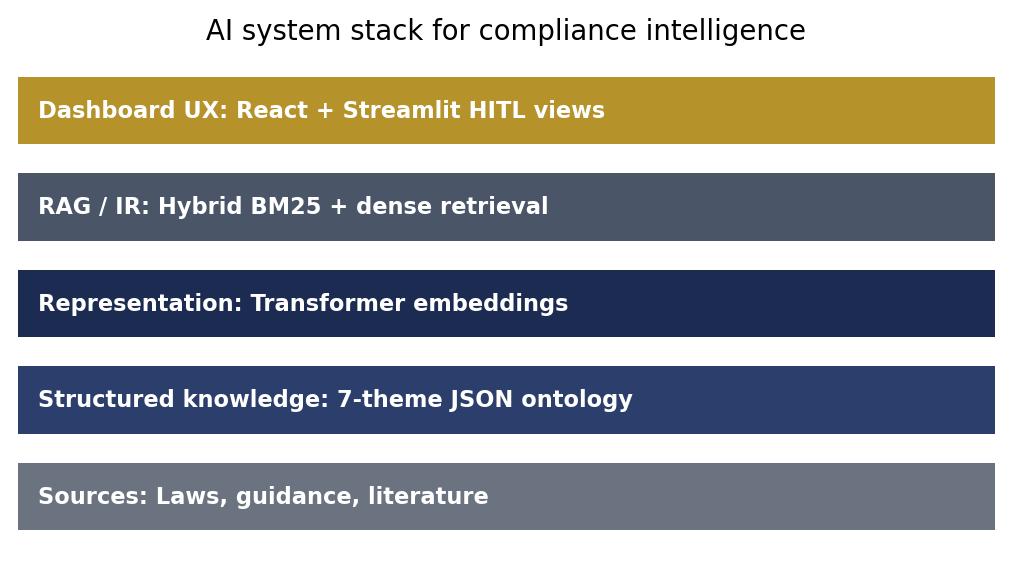
\includegraphics[width=\linewidth]{figures/fig_ai_system_stack.png}
\caption{Layered AI system stack used in this PFE.}
\label{fig:ai-stack}
\end{minipage}\hfill
\begin{minipage}[t]{0.48\textwidth}
\centering
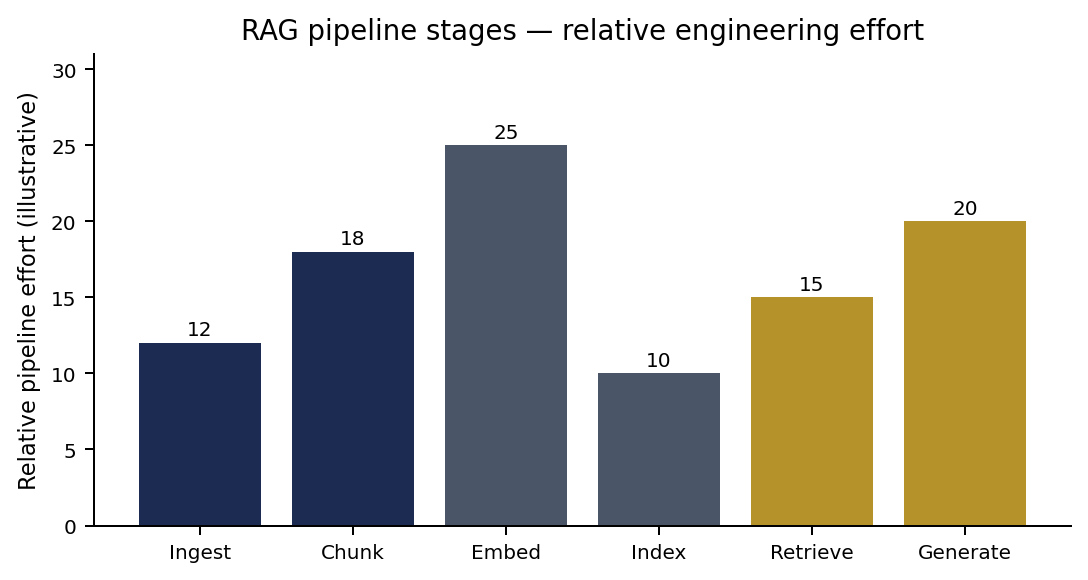
\includegraphics[width=\linewidth]{figures/fig_rag_pipeline_effort.png}
\caption{Illustrative relative engineering effort across RAG stages.}
\label{fig:rag-effort}
\end{minipage}
\end{figure}



\section{RAG Module Overview}
\label{sec:rag-overview-meth}

The Retrieval-Augmented Generation (RAG) module is the core information-retrieval
engine of the compliance platform. Its role in the overall pipeline is to transform
user queries into grounded, cited answers drawn exclusively from the indexed corpus
of regulatory sources. The design equation is

\begin{equation}
\hat{y} = g\!\left(q,\;\operatorname{TopK}_k(q,\mathcal{D})\right),
\end{equation}

where $q$ is the user query, $\mathcal{D}$ the corpus of indexed chunks, and $g$ the
citation-conditioned generator. The four-step contract is: \textbf{Corpus}
$\to$ \textbf{Retrieve} $\to$ \textbf{Generate} $\to$ \textbf{Dashboard}.

Because the RAG module constitutes an independent technical contribution, its full
architecture---corpus design, chunking, BM25 and dense indexing, Reciprocal Rank
Fusion, prompt engineering, HITL integration, evaluation framework, and code
implementation---is presented as a dedicated chapter. Refer to
Chapter~\ref{ch:rag} for the complete technical specification.

\section{Reproducibility, Validation, and Method Closing}
\label{sec:method-closing}

\subsection{Quality Assurance and Validity Threats}
\label{sec:qa}

Before cutting a dataset version:
\begin{enumerate}[noitemsep]
  \item schema validation (required keys, score ranges, ISO codes);
  \item cross-check legislation lists against narrative claims;
  \item spot-audit of extreme scores (10s and 1--2s) against primary sources;
  \item regenerate LaTeX score tables and visually inspect ranking shifts;
  \item smoke-test dashboard filters and CSV export round-trip.
\end{enumerate}
Construct validity threats include theme overlap (ethics vs transparency), imperfect mapping from ordinal scores to real enforcement, and the difficulty of encoding enforcement capacity. Internal validity threats include curator bias and drift over time. External validity threats include English-source bias, EU aggregation smoothing, and heterogeneous device-count definitions. Conclusion validity threats include over-reading authorization counts as quality proxies. The mitigation strategy is transparency: publish rubrics, narratives, version metadata, sensitivity checks (Section~\ref{sec:sensitivity}), and explicit non-legal-advice caveats so peers can contest and improve scores.

\subsection{Mapping Phase 1 Claims to Implemented Features}
\label{sec:phase1map}

Phase~1 promised a multi-level presentation from global map to compliance alerts, real-time monitoring, and HITL verification. Table~\ref{tab:phase1map} maps those claims to the current draft status.

\begin{table}[htbp]
\centering
\caption{Phase~1 ambitions versus draft implementation status}
\label{tab:phase1map}
\begin{tabular}{@{}p{4.2cm}p{3.0cm}p{4.0cm}@{}}
\toprule
\textbf{Phase~1 claim} & \textbf{Status} & \textbf{Notes} \\
\midrule
Comparative literature synthesis & Delivered & Thematic SotA + bibliography \\
Multi-country structured dataset & Delivered & 20 jurisdictions, 7 themes \\
Interactive dashboard (map/compare) & Delivered & Streamlit + React \\
NLP classification pipeline & Designed & Schema-ready; full training future \\
RAG hybrid retrieval module & Delivered (MVP) & Offline retriever + grounded UI \\
Real-time legislative monitoring & Roadmap & Versioned curation first \\
HITL verification & Delivered (process) & Manual score governance \\
\bottomrule
\end{tabular}
\end{table}

\subsection{Baseline Comparison Protocol for Analytics Claims}
\label{sec:baselineproto}

Guideline expectations for baselines are adapted to this analytics PFE as follows. The \textbf{null baseline} is an unweighted composite with no theme interpretation. The \textbf{literature baseline} is qualitative regime labeling from comparative studies (e.g., EU layered duties vs U.S.\ pathway throughput). The \textbf{alternative-weight baselines} are privacy-heavy, safety-heavy, and market-access-heavy recomputations of $S_c$. Claims in Chapter~\ref{ch:results} are accepted only when they survive at least one alternative weighting or match an independent literature characterization. Formal confidence intervals are not applicable to single-curator ordinal scores; instead, robustness is reported via rank stability under reweighting in Section~\ref{sec:sensitivity}.

\subsection{Mathematical Summary of Derived Indicators}
\label{sec:mathsummary}

Let $s_{c,t}$ denote the score of country $c$ on theme $t\in T$, $|T|=7$. The unweighted composite is
\begin{equation}
S_c=\frac{1}{|T|}\sum_{t\in T}s_{c,t}.
\end{equation}
A simple gap indicator used in results visualizations is
\begin{equation}
G_c^{\mathrm{priv-liab}}=s_{c,\mathrm{privacy}}-s_{c,\mathrm{liability}}.
\end{equation}
Use-case readiness scores apply fixed theme weights $w_{u,t}$ for use case $u$ (radiology, genomics, CDS, etc.):
\begin{equation}
R_{c,u}=\sum_{t\in T}w_{u,t}\,s_{c,t},\qquad \sum_{t}w_{u,t}=1.
\end{equation}
These formulae are intentionally transparent so that alternative weightings can be recomputed from exported CSV without reverse-engineering the UI.

\subsection{Methodological Conclusion}
\label{sec:methodconcl}

Methodology in this PFE is therefore a chain of justified choices: public sources, expert ordinal scoring, open JSON, interactive analytics, and an honest NLP roadmap. Extended runbook, ingestion, UI specification, and ethics-of-scoring notes are consolidated in Appendix~\ref{app:method}. Chapter~\ref{ch:rag} specifies the RAG module; Chapter~\ref{ch:results} reports empirical findings from the curated scores and dashboard views.


